%%%%%%%%%%%%%%%%%%%%%%%%%%%%%%%%%%%%%%%%%%%%%%%%%%%%%%%%%%%%%%%%%%%%%%%%%%%%%%%%
%% 
%%%%%%%%%%%%%%%%%%%%%%%%%%%%%%%%%%%%%%%%%%%%%%%%%%%%%%%%%%%%%%%%%%%%%%%%%%%%%%%%

\documentclass[a4paper, 12pt, oneside]{book}

%%-- Geometría principal (dejar activada la siguiente línea en la versión final)
\usepackage[a4paper, left=2.5cm, right=2.5cm, top=3cm, bottom=3cm]{geometry}
%%-- Activar esta línea y comentar la anterior en modo borrador, para comentarios al margen
%\usepackage[a4paper, left=2.5cm, right=2.5cm, top=3cm, bottom=3cm, marginparwidth=60pt]{geometry}

%%-- Hay que cargarlo antes que las traducciones
\usepackage{listing}                    % Listados de código

% Traducciones en XeLaTeX
\usepackage{polyglossia}
\setmainlanguage{spanish}    % Comenta esta línea si tu memoria es en inglés

% Traducciones particulares para español
% Caption tablas
\gappto\captionsspanish{
	\def\tablename{Tabla}
	\def\listingscaption{Código}
	\def\refname{Bibliografía}
	\def\appendixname{Apéndice}
	\def\listtablename{Índice de tablas}
	\def\listingname{Código}
	\def\listlistingname{Índice de fragmentos de código}
}

%% Tipografía y estilos
\usepackage[OT1]{fontenc}               % Keeps eulervm happy about accents encoding

% Símbolos y fuentes matemáticas elegantes: Euler virtual math fonts
% ¡Importante! Carga siempre las fuentes math AMS Euler ANTES QUE fontspec
\usepackage{amsmath}
\usepackage{amssymb}
\usepackage[OT1,euler-digits,euler-hat-accent,small]{eulervm}

% En XeLaTeX las fuentes se especifican con fontspec
\usepackage{fontspec}
\defaultfontfeatures{Scale=MatchLowercase, Ligatures=TeX}     % Default option in font config

% Fix para fuentes usadas con operadores y \mathrm
\DeclareSymbolFont{operators}{\encodingdefault}{\familydefault}{m}{n}

% Configura la fuente principal (serif): MinionPro
\setmainfont[Scale=0.96]{TeX Gyre Pagella}
% Configura la fuente sans-serif (\sffamily)
\setsansfont[Scale=MatchLowercase]{Lato}
% Configura la fuente para letra monoespaciada: Source Code Pro, escala 0.85
\setmonofont[Scale=0.85]{Source Code Pro}

%%-- Familias de fuentes específicas
%%-- Se pueden definir etiquetas para familias de fuentes personalizadas
%%-- que luego puedes emplear para cambiar el formato de una parte de texto
%%-- Ejemplo:
% \newfontfamily{\myriadprocond}{Myriad Pro Semibold Condensed.otf}

%%-- Opciones de interlineado y espacios
\linespread{1.07}                   % Aumentar interlineado para fuentes tipo Palatino
\setlength{\parskip}{\baselineskip} % Separar párrafos con línea en blanco

% Line and page breaking
\sloppy
\clubpenalty = 10000
\widowpenalty = 10000
\brokenpenalty = 10000
\usepackage{ragged2e}				% Enhanced ragged commands

%%-- Hipervínculos
\usepackage{url}

%%-- Gráficos y tablas
\PassOptionsToPackage{dvipdfmx,usenames,dvipsnames,x11names,table}{xcolor}             % Definiciones de colores
\PassOptionsToPackage{xetex}{graphicx}

\usepackage{subfig}                     % Subfiguras
\usepackage{pgf}
\usepackage{svg}                        % Integración de imágenes en formato SVG
\usepackage{float}                      % H para posicionar figuras
\usepackage{booktabs}                   % Already loads package xcolor
\usepackage{longtable}                  % Tables spanning several pages
\usepackage{multicol}                   % multiple column layout facilities
\usepackage{colortbl}                   % For coloured tables
\usepackage{array}                      % Column adjustment in tables

%%-- Bibliografía con Biblatex y Biber
% Más info:
% https://www.overleaf.com/learn/latex/Biblatex_bibliography_styles
% https://www.overleaf.com/learn/latex/biblatex_citation_styles
\usepackage[
    backend=biber,
    style=numeric,
    sorting=none
    ]{biblatex}
\addbibresource{memoria.bib}
% \DeclareFieldFormat{url}{\mkbibacro{URL}\addcolon\nobreakspace\url{#1}}
%\usepackage[nottoc, notlot, notlof, notindex]{tocbibind} %% Opciones de índice

%%-- Matemáticas e ingeniería
% El paquete units permite mostrar unidades correctamente
% Permite escribir unidades con espaciado y estilo de fuente correctos
\usepackage{units}         
% Ejemplo de uso: $\unit[100]{m}$ or $\unitfrac[100]{m}{s}$
% Entornos matemáticos
\newtheorem{theorem}{Theorem}

% Paquetes adicionales
\usepackage{url}                        %% Gestión correcta de enlaces
\usepackage{float}                      %% H para posicionar figuras
\usepackage[nottoc, notlot, notlof, notindex]{tocbibind}    %% Opciones de índice
\usepackage{metalogo}                   %% Múltiples logos para XeLaTeX

% Fuentes especiales y glifos
\usepackage{ccicons}                % Creative Commons icons
\usepackage{metalogo}               % XeTeX logo
\usepackage{fontawesome5}           % Fontawesome 5 icons
\usepackage{adforn} 

% Blindtext
% Opciones pangram, bible, random (defecto)
\usepackage[pangram]{blindtext}
% Lorem ipsum
\usepackage{lipsum}
% Kant lipsum
\usepackage{kantlipsum}

\usepackage{fancyvrb}               % Entornos verbatim extendidos
	\fvset{fontsize=\normalsize}    % Tamaño de fuente por defecto en fancy-verbatim
	
% Configura listas (itemize, enumerate) con iconos personalizados
% Fácil reinicio de numeración con enumerate
% Info: http://ctan.org/pkg/enumitem
\usepackage[shortlabels]{enumitem}
% Usar \usageitem para configurar iconos personalizados en listas
\newcommand{\usageitem}[1]{%
	\item[%
	{\makebox[2em]{\strut\color{GSyCblue} #1}}%
	]
}

%%-- Definición de colores personalizados
% \definecolor{LightGrey}{HTML}{EEEEEE}
% \definecolor{darkred}{rgb}{0.5,0,0}     %% Refs. cruzadas
% \definecolor{darkgreen}{rgb}{0,0.5,0}   %% Citas bibliográficas
% \definecolor{darkblue}{rgb}{0,0,0.5}    %% Hiperenlaces ordinarios (también ToC)

%%-- Configuración fragmentos de código
%%-- Minted necesita Python Pygments instalado en el sistema para funcionar
%%-- En Overleaf ya está instalada esta dependencia
\usepackage[labelfont=bf]{caption}
\newcommand{\source}[1]{\vspace{-3pt} \caption*{Fuente: {#1}} }
\usepackage{minted}
\usemintedstyle{vs}

%%-- Se debe cargar aquí para evitar warnings
\usepackage{csquotes}                   % Para traducciones con biblatex

%%-- Glosario de términos
\usepackage[acronym]{glossaries}
\makeglossaries
\loadglsentries{glossary}

% % Definición de cabeceras del documento, usando fancyhdr
% \usepackage{fancyhdr}
% %% Configuración de cabeceras para el cuerpo principal del documento
% \pagestyle{fancy}
% \fancyhead{}
% \fancyhead[RO,LE]{\myriadprocond{\thepage}}
% \renewcommand{\chaptermark}[1]{\markboth{\chaptername\ \thechapter.\ #1}{}}
% \renewcommand{\sectionmark}[1]{\markright{\thesection.\ #1}}
% \fancyhead[RE]{\myriadprocond{\leftmark}}
% \fancyhead[LO]{\myriadprocond{\rightmark}}
% \renewcommand{\headrulewidth}{0pt}
% \setlength{\headheight}{15pt} %% Al menos 15pt para evitar warning al compilar
% \fancyfoot{}
% %% Configuración para páginas con cabecera en blanco
% \fancypagestyle{plain}{%
% \fancyhf{}% clear all header and footer fields
% \fancyhead[RO,LE]{\myriadprocond{\thepage}}
% \renewcommand{\headrulewidth}{0pt}%
% \renewcommand{\footrulewidth}{0pt}%
% }
\AtBeginDocument{\addtocontents{toc}{\protect\thispagestyle{empty}}} 

%%%%%%%%%%%%%%%%%%%
%% Own changes
%%%%%%%%%%%%%%%%%%%
\newenvironment{conditions}[1][donde:]
  {#1 \begin{tabular}[t]{>{$}l<{$} @{${}={}$} l}}
  {\end{tabular}\\[\belowdisplayskip]}
\raggedbottom


%%%%%%%%%%%%%%%%%%%%%%%%%%%%%%%%%%%%%%%%

%%-- Metadatos del doc
\title{Comparativa del Consumo Energético de Algoritmos de Aprendizaje Automático}
\author{Laura Gonzalez Fernandez}

%%-- Hiperenlaces, siempre se carga al final del preámbulo
\usepackage[colorlinks]{hyperref}
\hypersetup{
    pdftoolbar=true,	% Muestra barra de herramientas en Adobe Acrobat
	pdfmenubar=true,	% Muestra menú en Adobe Acrobat
	pdftitle={TFG - Comparativa del Consumo Energético de Algoritmos de Aprendizaje Automático},
	pdfauthor={Laura Gonzalez Fernandez},
	pdfcreator={EIF, URJC},
	pdfproducer={XeLaTeX},
	pdfsubject={Machine-learning, eficiencia energética},
	pdfnewwindow=true,              %links open in new window
    colorlinks=true,                % false: boxed links; true: coloured links
    linkcolor=Firebrick4,           % enlaces internos 
    citecolor=Aquamarine4,          % enlaces a citas bibliográficas
    urlcolor=RoyalBlue3,            % hiperenlances ordinarios
    linktocpage=true                % Enlaces en núm. pág. en ToC
}

%%%---------------------------------------------------------------------------
% Comentarios en línea de revisión
% Este bloque se puede borrar cuando finalizamos el borrador

\usepackage[colorinlistoftodos]{todonotes}
\newcommand\todoin[2][]{\todo[inline, color=green!40, caption={2do}, #1]{
\begin{minipage}{\textwidth-4pt}#2\end{minipage}}}
\usepackage{verbatim}

% \hyphenpenalty 10
% \exhyphenpenalty 10
\pretolerance=5000
\tolerance=9000
\emergencystretch=2pt
\righthyphenmin=4
\lefthyphenmin=4

\interfootnotelinepenalty=10000

\usepackage[
    type={CC},
    modifier={by-sa},
    version={4.0},
]{doclicense}

%%%---------------------------------------------------------------------------

\begin{document}

%%-- Configuración común para todos los entornos listing
%%-- Descomentar para usar y personalizar valores
%\lstset{%
%breakatwhitespace=true,
% breaklines=true, 
% basicstyle=\footnotesize\ttfamily,
% keywordstyle=\color{blue},
% commentstyle=\color{green!40!black}, 
% language=Python} 
 

%%%%%%%%%%%%%%%%%%%%%%%%%%%%%%%%%%%%%%%%%%%%%%%%%%%%%%%%%%%%%%%%%%%%%%%%%%%%%%%%
% PORTADA

\begin{titlepage}
\begin{center}
\begin{tabular}[c]{c c}
%\includegraphics[bb=0 0 194 352, scale=0.25]{logo} &
\includegraphics[scale=1.5]{img/LogoURJC.png}
%&
%\begin{tabular}[b]{l}
%\Huge
%\textsf{UNIVERSIDAD} \\
%\Huge
%\textsf{REY JUAN CARLOS} \\
%\end{tabular}
\\
\end{tabular}

\vspace{1.5cm}

\Large 
ESCUELA DE INGENIERÍA DE FUENLABRADA

\vspace{1.2cm}

\Large 
GRADO EN INGENIERÍA EN TECNOLOGÍAS DE LA TELECOMUNICACIÓN

\vspace{0.8cm}
\LARGE 
\textbf{\uppercase{Trabajo Fin de Grado}}

\vspace{2cm}

\LARGE Comparativa de modelos de aprendizaje automático con respecto a su consumo energético
\vspace{2cm}

\large
Autora : Laura González Fernández \\
Tutor : José Felipe Ortega Soto

\vspace{0.8cm}
\large
Curso Académico 2023/2024

\end{center}
\pagenumbering{gobble}
\end{titlepage}


\newpage
\mbox{}


%%%%%%%%%%%%%%%%%%%%%%%%%%%%%%%%%%%%%%%%%%%%%%%%%%%%%%%%%%%%%%%%%%%%%%%%%%%%%%%%
%%%% Para firmar
\clearpage
\frontmatter
\pagestyle{empty}
\chapter*{}
\thispagestyle{empty}

\vspace{-4cm}
\begin{center}
\LARGE
\textbf{Trabajo Fin de Grado}

\vspace{1cm}
\large
Comparativa del Consumo Energético de Algoritmos de Aprendizaje Automático

\vspace{1cm}
\large
\textbf{Autora :} Laura González Fernández  \\
\textbf{Tutor :} José Felipe Ortega Soto

\end{center}

\vspace{1cm}
La defensa del presente Proyecto Fin de Grado se realizó el día \qquad$\;\,$ de \qquad\qquad\qquad\qquad \newline de 2024, siendo calificada por el siguiente tribunal:


\vspace{0.5cm}
\textbf{Presidente:}

\vspace{0.8cm}
\textbf{Secretario:}

\vspace{0.8cm}
\textbf{Vocal:}


\vspace{0.8cm}
y habiendo obtenido la siguiente calificación:

\vspace{0.8cm}
\textbf{Calificación:}


\vspace{0.8cm}
\begin{flushright}
Fuenlabrada, a \qquad$\;\,$ de \qquad\qquad\qquad\qquad de 2024
\end{flushright}

%%%%%%%%%%%%%%%%%%%%%%%%%%%%%%%%%%%%%%%%%%%%%%%%%%%%%%%%%%%%%%%%%%%%%%%%%%%%%%%%
%%%% Dedicatoria

% \chapter*{}
% \thispagestyle{empty}
% %\pagenumbering{Roman} % para comenzar la numeración de paginas en numeros romanos
% \begin{flushright}
% \textit{To the future.\\}
% \end{flushright}

\chapter*{}
\thispagestyle{empty}
%\pagenumbering{Roman} % para comenzar la numeración de paginas en numeros romanos

\begin{flushright}
\begin{minipage}{8cm}
\raggedleft
©2024 Laura González Fernández  \\
Algunos derechos reservados. \\
\doclicenseLongText \\
\vspace{0.5cm}
\doclicenseImage
\end{minipage}

\end{flushright}

%%%%%%%%%%%%%%%%%%%%%%%%%%%%%%%%%%%%%%%%%%%%%%%%%%%%%%%%%%%%%%%%%%%%%%%%%%%%%%%%
%%%% Agradecimientos

\chapter*{Agradecimientos}
\thispagestyle{empty}
%\addcontentsline{toc}{chapter}{Agradecimientos} % si queremos que aparezca en el índice
\markboth{AGRADECIMIENTOS}{AGRADECIMIENTOS} % encabezado 

% I would like to take this opportunity to express my deepest gratitude to the many individuals who have played a significant role in the completion of this bachelor thesis.

% First and foremost, I want to thank my family for their unwavering support and patience throughout my academic journey. They never doubted me, even when I did it myself. Thank you as well for your help during this project, for being there when I needed a camera person or an extra hand to fly the drone. To my sister, especially, thank you for putting up with me these two years while I inched along this project.

% I also extend my thanks to my supervisors for their guidance, expertise, and invaluable feedback throughout the thesis project. Your dedication to my academic growth and your willingness to share your knowledge have been indispensable.

% I would also like to express my gratitude to all my friends and colleagues who were by my side during this journey. Your camaraderie and the frequent inquiries about the status of my "never-ending drone project" pushed me towards the finish line.

% This thesis represents the culmination of years of hard work and dedication, and I am grateful for the support of everyone who stood by my side.

% Thank you all for being a part of this journey.

%%%%%%%%%%%%%%%%%%%%%%%%%%%%%%%%%%%%%%%%%%%%%%%%%%%%%%%%%%%%%%%%%%%%%%%%%%%%%%%%
%%%% Resumen

\chapter*{Resumen}
\thispagestyle{empty}
%\addcontentsline{toc}{chapter}{Resumen} % si queremos que aparezca en el índice
\markboth{RESUMEN}{RESUMEN} % encabezado
%(máximo una página, se recomienda la estructura: antecedentes,
%objetivos, métodos, resultados y conclusiones)

Aquí viene un resumen del proyecto.
Ha de constar de tres o cuatro párrafos, donde se presente de manera clara y concisa de qué va el proyecto. 
Han de quedar respondidas las siguientes preguntas:

\begin{itemize}
  \item ¿De qué va este proyecto? ¿Cuál es su objetivo principal?
  \item ¿Cómo se ha realizado? ¿Qué tecnologías están involucradas?
  \item ¿En qué contexto se ha realizado el proyecto? ¿Es un proyecto dentro de un marco general?
\end{itemize}

Lo mejor es escribir el resumen al final.
\\\noindent\rule{\textwidth}{0.4pt}
Intro provisional:

El aprendizaje automático se ha desarrollado a pasos de gigante durante los últimos años y sus avances han permitido que los sistemas informáticos sean capaces de abstraer relaciones entre objetos y hacer predicciones sobre el futuro. Pero los grandes proyectos de aprendizaje requieren de la utilización de grandes cantidades de datos y los correspondientes potentes procesadores que sean capaces de trabajar con ellos. En el panorama actual cada vez más se vuelve una responsabilidad ser consciente de la huella causada en el medio ambiente por el consumo energético de los ordenadores.

Con este proyecto se pretende proporcionar una herramienta capaz de comparar entre los modelos más comunes empleados en aprendizaje automático, que pueda dar respuesta a la preocupación de equilibrar la precisión y eficacia de los modelos de aprendizaje con su impacto desde el punto de vista energético. Para ello se utilizarán las herramientas proporcionadas por Scikit-learn, Python y Codecarbon y conjuntos de datos representativos disponibles públicamente en la web con licencia abierta.


%%%%%%%%%%%%%%%%%%%%%%%%%%%%%%%%%%%%%%%%%%%%%%%%%%%%%%%%%%%%%%%%%%%%%%%%%%%%%%%%
%%%% Resumen en inglés

\chapter*{Summary}
%\addcontentsline{toc}{chapter}{Summary} % si queremos que aparezca en el índice
\markboth{SUMMARY}{SUMMARY} % encabezado

Here comes a translation of the ``Resumen'' into English. 
Please, double check it for correct grammar and spelling.
As it is the translation of the ``Resumen'', which is supposed to be written at the end, this as well should be filled out just before submitting.

%%%%--------------------------------------------------------------------
% Lista de comentarios de revisión
% Se puede borrar este bloque al acabar el borrador

\listoftodos
\thispagestyle{empty}
\markboth{TODO LIST}{TODO LIST} % encabezado
%%%%--------------------------------------------------------------------

%%%%%%%%%%%%%%%%%%%%%%%%%%%%%%%%%%%%%%%%%%%%%%%%%%%%%%%%%%%%%%%%%%%%%%%%%%%%%%%%
%%%%%%%%%%%%%%%%%%%%%%%%%%%%%%%%%%%%%%%%%%%%%%%%%%%%%%%%%%%%%%%%%%%%%%%%%%%%%%%%
% ÍNDICES %
%%%%%%%%%%%%%%%%%%%%%%%%%%%%%%%%%%%%%%%%%%%%%%%%%%%%%%%%%%%%%%%%%%%%%%%%%%%%%%%%

% Las buenas noticias es que los índices se generan automáticamente.
% Lo único que tienes que hacer es elegir cuáles quieren que se generen,
% y comentar/descomentar esa instrucción de LaTeX.

%%-- Índice de contenidos
\tableofcontents 
\thispagestyle{empty}
\cleardoublepage
%%-- Índice de figuras

\addcontentsline{toc}{chapter}{Lista de figuras} % para que aparezca en el indice de contenidos
\thispagestyle{empty}
\listoffigures % indice de figuras
\thispagestyle{empty}

\cleardoublepage
%%-- Índice de tablas
%\addcontentsline{toc}{chapter}{Lista de tablas} % para que aparezca en el indice de contenidos
%\listoftables % indice de tablas
% \cleardoublepage
%%-- Índice de fragmentos de código
% \addcontentsline{toc}{chapter}{List of listings} % para que aparezca en el indice de contenidos
% \listoflistings

%%%%%%%%%%%%%%%%%%%%%%%%%%%%%%%%%%%%%%%%%%%%%%%%%%%%%%%%%%%%%%%%%%%%%%%%%%%%%%%%
%%%%%%%%%%%%%%%%%%%%%%%%%%%%%%%%%%%%%%%%%%%%%%%%%%%%%%%%%%%%%%%%%%%%%%%%%%%%%%%%
%%%%%%%%%%%%%%%%%%%%%%%%%%%%%%%%%%%%%%%%%%%%%%%%%%%%%%%%%%%%%%%%%%%%%%%%%%%%%%%%
%%%%%%%%%%%%%%%%%%%%%%%%%%%%%%%   CONTENT   %%%%%%%%%%%%%%%%%%%%%%%%%%%%%%%%%%%%
%%%%%%%%%%%%%%%%%%%%%%%%%%%%%%%%%%%%%%%%%%%%%%%%%%%%%%%%%%%%%%%%%%%%%%%%%%%%%%%%
%%%%%%%%%%%%%%%%%%%%%%%%%%%%%%%%%%%%%%%%%%%%%%%%%%%%%%%%%%%%%%%%%%%%%%%%%%%%%%%%
%%%%%%%%%%%%%%%%%%%%%%%%%%%%%%%%%%%%%%%%%%%%%%%%%%%%%%%%%%%%%%%%%%%%%%%%%%%%%%%%
\mainmatter
\pagestyle{headings}

%\cleardoublepage
\chapter{Introducción}
\label{sec:intro}
\pagenumbering{arabic} 

El aprendizaje automático (\emph{machine learning} o ML en inglés) es una rama de la Inteligencia Artificial y las Ciencias de la Computación que se centra en el uso de datos y algoritmos para imitar la forma en la que los humanos aprenden con el objetivo de aumentar gradualmente su precisión.
Es un componente fundamental del campo de la Ciencia de Datos, cuya importancia ha experimentado un gran crecimiento, especialmente en las últimas dos décadas \cite{cleveland2001}. 
El aprendizaje automático hace uso de métodos estadísticos y computacionales para entrenar algoritmos que realizan, entre otras tareas, clasificaciones o predicciones y que permiten descubrir piezas clave de información dentro de proyectos de procesamiento de datos. 
Posteriormente, esta información puede utilizarse en la toma de decisiones dentro de distintas aplicaciones y negocios, con una gran capacidad de impactar en el crecimiento de los mismos.

\section{Aprendizaje automático y consumo energético}

Gracias al desarrollo de nuevas tecnologías computacionales, el aprendizaje automático que se utiliza hoy en día es muy diferente de como era en el pasado.
El modelo actual surgió del reconocimiento de patrones y de la teoría de que los ordenadores pueden aprender a resolver tareas específicas, cuando los investigadores interesados en la Inteligencia Artificial se empezaron a plantear si los ordenadores serían capaces de aprender a partir de datos.
De aquí surge la importancia del aspecto iterativo de este aprendizaje, que permite que el sistema se adapte de forma independiente cada vez que nuevos datos son incorporados y sea capaz de aprender de cada computación previa para producir decisiones y resultados que sean confiables y repetibles.

Es así que, aunque una gran parte de los algoritmos utilizados en el aprendizaje automático son conocidos desde hace relativamente bastante tiempo, la habilidad de aplicar complejos cálculos matemáticos a grandes cantidades de datos una y otra vez, cada vez más rápidamente, es un desarrollo muy reciente conseguido gracias a los avances en componentes informáticos y la disminución de costes de grandes sistemas computacionales con enormes capacidades de memoria y procesamiento.
En especial, esto sucede en el campo del aprendizaje profundo (\emph{deep learning}), donde los modelos han crecido en cálculos para llegar a alcanzar típicamente el orden de los GigaFlops y en requisitos de memoria que se encuentran comúnmente en el orden de los millones de parámetros.

Sin embargo, este gran poder de procesamiento también trae consigo un gran gasto energético.
El consumo de energía en la arquitectura de computadores ha sido foco de atención de investigadores interesados en obtener procesadores energéticamente eficientes de última generación durante décadas. 
Por otro lado, los investigadores interesados en el aprendizaje automático se han centrado principalmente en la producción de modelos cada vez más profundos y precisos, sin poner ningún límite en términos computacionales más allá de la disponibilidad de procesadores capaces de llevar a cabo estos cálculos.

\begin{figure}[H]
  \centering
  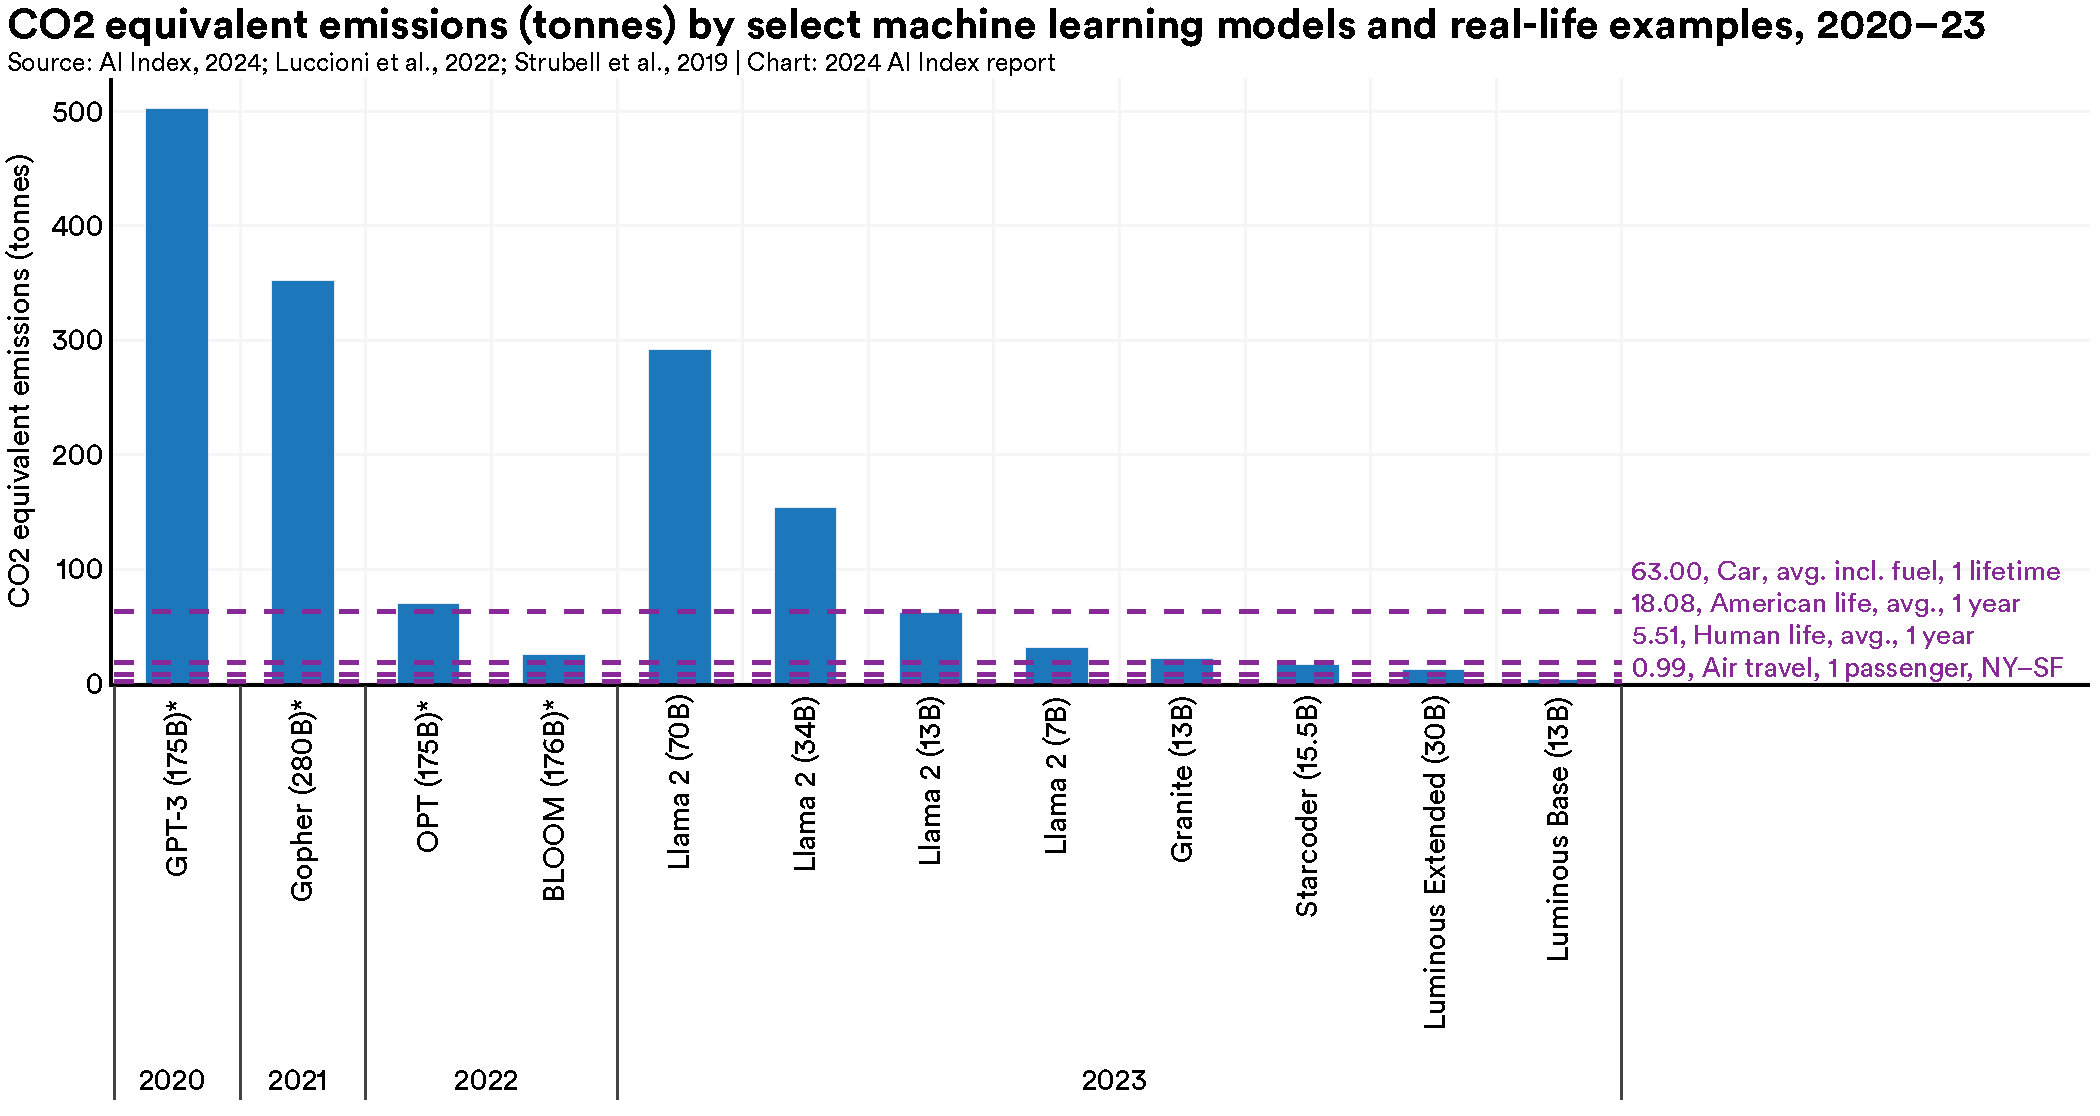
\includegraphics[width=\textwidth,keepaspectratio]{img/fig_2.13.1-ai-index.pdf}
  \caption{Emisiones de $CO_2$ producidas en el entrenamiento de varios modelos de gran escala en los últimos años. \\ Fuente: \citetitle{maslej2024aiindex} \cite{maslej2024aiindex}.}
  \label{fig:ai-index-emissions}
\end{figure}

Adicionalmente, con la reciente popularización de los grandes modelos de aprendizaje, especialmente de los modelos de lenguaje de gran escala (\textit{Large Language Models}, LLMs), pero también de la visión por computador y el aprendizaje en la nube, la investigación sobre el impacto energético se hace aún más necesaria. Los grandes modelos de lenguaje, por ejemplo, requieren enormes cantidades de datos y recursos computacionales para su entrenamiento, lo que se traduce en un consumo energético considerable \cite{samsi2023}. \mbox{GPT-3} \cite{brown2020language}, uno de los modelos más conocidos, cuenta con 175 mil millones de parámetros y requiere una cantidad masiva de energía para su entrenamiento. Del mismo modo, las aplicaciones de visión por computador, especialmente aquellas que involucran redes convolucionales profundas (CNN), también son intensivas en energía \cite{alyamkin2019low}. La figura~\ref{fig:ai-index-emissions} muestra las emisiones de $CO_2$ estimadas producidas durante el entrenamiento de varios modelos recientes, comparadas con referencias comunes como el consumo medio por una persona durante toda su vida.

El aprendizaje en la nube agrava estos problemas al trasladar el consumo energético a los centros de datos, que pueden tener diferentes niveles de eficiencia y fuentes de energía. Este tipo de aprendizaje, aunque ofrece flexibilidad y escalabilidad, puede tener implicaciones negativas para el consumo energético. Los centros de datos que alimentan estos servicios requieren grandes cantidades de electricidad, y su impacto depende en gran medida de la fuente de energía utilizada. Algunos centros de datos están migrando hacia fuentes de energía renovable para mitigar este impacto, pero la transición no es uniforme en todas las regiones.


\section{Desarrollo de una aplicación comparativa: \emph{MLCost}}

En este contexto temporal de modelos de aprendizaje que cada vez consumen más energía, se hace más necesario que nunca contar con una medida de la energía consumida y las emisiones producidas durante el proceso de entrenamiento. Esta información es vital para poder realizar una decisión informada en la elección de que modelos utilizar para una aplicación concreta de aprendizaje automático. Este proyecto propone el desarrollo de una aplicación, con el nombre MLCost, que permita a los investigadores obtener esta información de forma sencilla mediante el uso de herramientas existentes de medición. Para ello, la aplicación hace uso de librerías como CodeCarbon, que permite abstraer el método de calculo de emisiones, y Scikit-Learn, que permite entrenar modelos sin considerar gran parte del desarrollo de bajo nivel asociado con la implementación de los algoritmos utilizados y la preparación de conjuntos de datos para el entrenamiento. De este modo, la aplicación posibilita la medición del consumo y las emisiones producidas por distintos modelos a estudiar en cualquier conjunto de datos que se quiera utilizar, así como la comparación con gráficos sencillos de los resultados obtenidos.


\section{Objetivos del proyecto}
\label{sec:objetivos}

\subsection{Objetivo general}
\label{sec:objetivo-general}


Este Trabajo de Fin de Grado tiene como objetivo crear una herramienta que permita la comparación sistemática del consumo energético y el impacto de la huella de carbono en los modelos más representativos de técnicas de clasificación de aprendizaje automático supervisado.


\subsection{Objetivos específicos}
\label{sec:objetivos-especificos}

Para esta finalidad se han tenido en cuenta los siguientes objetivos específicos:

    \begin{itemize}
        \item Estudiar las herramientas disponibles para aprendizaje automático.
        \item Estudiar el uso de herramientas de medida del consumo energético.
        \item Comparar el consumo energético en los algoritmos de clasificación más importantes.
        \item Analizar la relación entre la precisión de los modelos y su consumo energético en conjuntos de datos de distintos tamaños y características.
    \end{itemize}

\section{Estructura de la memoria}
\label{sec:estructura}

La memoria de este proyecto se estructura en cinco capítulos, con una introducción, seguida de tres capítulos que reflejan las tres fases principales del proyecto: investigación, desarrollo y validación, para finalizar con las conclusiones y trabajos futuros.

El primer capítulo introduce el contexto en el cual se ha desarrollado la aplicación, proporcionando información de fondo y destacando los objetivos principales del proyecto. Este capítulo establece el escenario para los capítulos siguientes, ofreciendo una visión general del alcance y propósito del proyecto.

El segundo capítulo revisa la literatura relevante y el estado del arte en cuanto a métodos de medición de emisiones y estudios sobre el consumo energético del aprendizaje automático. Además, proporciona una introducción general al aprendizaje automático, describe las librerías existentes utilizadas en el desarrollo del proyecto y detalla los modelos y conjuntos de datos utilizados durante las pruebas de la aplicación.

El tercer capítulo describe la arquitectura de la aplicación desarrollada, incluyendo el proceso de preparación de los datos y los métodos de evaluación de las predicciones de los modelos. Este capítulo se centra en los aspectos técnicos del diseño y la implementación, explicando las decisiones de diseño y cómo se implementaron las diferentes funcionalidades.

El cuarto capítulo recoge todas las pruebas realizadas con la aplicación, incluyendo dos experimentos concretos. El primero compara varios modelos en distintos conjuntos de datos de creciente complejidad, mientras que el segundo compara varios modelos en diferentes máquinas con diversos recursos de procesamiento. Este capítulo detalla la metodología de los experimentos y presenta los resultados obtenidos, analizando el impacto del consumo energético en el rendimiento de los modelos.

El último capítulo concluye la memoria resumiendo los principales hallazgos del proyecto y evaluando el grado de consecución de los objetivos planteados. Además, este capítulo incluye una reflexión sobre el conocimiento adquirido y sugiere posibles direcciones para trabajos futuros, proponiendo mejoras y ampliaciones a los estudios realizados.

%\cleardoublepage
\chapter{Estado del arte}
\label{chap:sota}

\section{Revisión de la literatura}
\label{sec:lit-rev}

\todoin{
Literature review: \\
  > Codecarbon paper \\
  > Research projects into machine learning consumption \\
  > Métodos que han utilizado y resultados \\
  > ChatGPT, LLM, computer vision, cloud, etc. how much energy?
}

\section{Aprendizaje automático}
\label{sec:intro-ml}

\todoin{Mini intro to machine learning:  \\
  > supervised vs unsupervised \\
  > classification vs regression \\
  > modelos vs redes neuronales \\
  > features vs labels \\
  > train vs test \\
  > types of features}

\section{Librerías empleadas}

\subsection{Entorno de desarrollo}
\label{sec:dev-env}

\todo[inline]{VSCode + WSL}


\subsection{Codecarbon}

CodeCarbon es un paquete creado con la intención de permitir a desarrolladores monitorizar las emisiones de dióxido de carbono ($CO_{2}$) producidas por aplicaciones en Inteligencia Artificial y modelos de Aprendizaje Automático, que surge de la motivación de contar con una forma de registrar las enormes cantidades de energía que el auge de la IA ha provocado en la industria. El incremento del rendimiento y la precisión de los modelos de Aprendizaje Automático que se ha producido en años recientes se ha logrado a cambio de la utilización de enormes cantidades de información para conseguir el aprendizaje de los patrones y características subyacentes. Así, los modelos más avanzados emplean cantidades significativas de poder computacional, entrenando en procesadores avanzados durante semanas o meses y consumiendo en el proceso una gran cantidad de energía. Dependiendo de la red eléctrica utilizada, este desarrollo puede comportar la emisión de grandes cantidades de gases de efecto invernadero como el $CO_{2}$.

CodeCarbon estima la huella de carbono de una aplicación medida como kilogramos de $CO_{2}$ equivalentes, o $CO_{2}eq$, una medida estandarizada utilizada para expresar la capacidad de calentamiento global de varios gases de efecto invernadero como la cantidad de $CO_{2}$ que causaría un impacto ambiental equivalente. Para tareas de computación, que emiten $CO_{2}$ por medio de la electricidad que están consumiendo y que es generada como parte de la red eléctrica (por ejemplo, mediante la quema de combustibles fósiles como el carbón) las emisiones de carbono se miden en kilogramos de $CO_{2}$ equivalentes por kilovatio-hora. De esta forma, las emisiones de dióxido de carbono totales se calculan como el producto de la intensidad de carbono de la electricidad utilizada para la computación y la energía consumida por la infraestructura.

La intensidad de carbono de la electricidad se calcula como la media ponderada de las emisiones de las distintas fuentes de energía usadas para generar electricidad, incluyendo combustibles fósiles y renovables. En la herramienta se asigna un valor conocido de dióxido de carbono emitido por kilovatio-hora generado para cada uno de los combustibles (carbón, petróleo y gas natural). Otras fuentes renovables o consideradas como de bajo carbono incluyen la energía solar, hidroeléctrica, biomasa o geotérmica. La intensidad de carbono de cada combustible individual se calcula en base a medidas de generación de carbono y electricidad en los Estados Unidos, y aplicadas de forma generalizada en el resto del mundo. Cada red eléctrica local incluye una mezcla distinta de fuentes de energía y tiene asignada entonces una intensidad de carbono total particular.

% IMAGE: Global distribution of carbon intensity (carbonboard)
% TABLE: Carbon intensity by energy source (Codecarbon/Methodology)
% CITE: CodeCarbon documentation

% _opcional_ : explanation on zero value for low-carbon fuels
% _opcional_ : explanation on power consuption calculation by CPU

\subsection{Scikit-Learn}

Scikit-learn es un módulo desarrollado para Python que integra un amplio rango de algoritmos de aprendizaje automático de última generación para problemas tanto supervisados como no supervisados. Este paquete pretende llevar el aprendizaje automático a desarrolladores no especialistas mediante el uso de un lenguaje generalista de alto nivel. Se hace hincapié en la facilidad de uso, el rendimiento, la documentación y la consistencia de la API. Tiene las mínimas dependencias necesarias y está distribuido bajo la licencia BSD, con el objetivo de incentivar su uso tanto en ambientes educativos como comerciales.

Scikit-learn expone una gran variedad de algoritmos de aprendizaje utilizando una interfaz consistente y orientada a la resolución de tareas, lo que permite una comparación sencilla entre distintos métodos de aprendizaje para una misma aplicación. Al depender del ecosistema científico de Python, puede ser integrado con facilidad en aplicaciones que se salgan del rango tradicional del análisis estadístico de datos. Además, los algoritmos, que han sido implementados en un lenguaje de alto nivel, pueden ser utilizados como bloques de construcción para desarrollar estrategias más complejas que se adecuen a cada caso particular.

\todo[inline]{CITE: Scickit-learn/About}

\subsection{Matplotlib / Altair}

\todo[inline]{Graphics libraries}

%%%%
%% ALGORITHMS, CURRENTLY
%%%%

\section{Modelos utilizados}
\label{sec:models}

\subsection{Modelos lineales: regresión logística}

Los modelos lineales son una clase fundamental de técnicas estadísticas y de aprendizaje automático que se utilizan para predecir una variable objetivo a partir de una o más variables independientes. La característica principal de estos modelos es la relación lineal entre las variables independientes y la variable objetivo. En su forma más simple, el modelo lineal se representa mediante la ecuación $y = \beta_0 + \beta_1 x_1 + \beta_2 x_2 + \dots + \beta_n x_n$, donde $y$ es la variable dependiente, $x_1, x_2, \dots, x_n$ son las variables independientes, y $\beta_1, \beta_2, \dots, \beta_n$ son los coeficientes que representan el impacto de cada variable independiente sobre la variable dependiente.

Dentro de los modelos lineales, la regresión logística es especialmente relevante para problemas de clasificación. A diferencia de la regresión lineal, que se utiliza para problemas de predicción continua, la regresión logística se emplea cuando la variable objetivo es categórica. En su forma binaria más simple, la regresión logística predice la probabilidad de que una observación pertenezca a una de dos posibles categorías. La función logística o sigmoide, 
\begin{equation*}
    P(y=1\mid x) = \frac{1}{1+e^{-\beta_0 + \beta_1 x_1 + \beta_2 x_2 + \dots + \beta_n x_n}},
\end{equation*}
transforma cualquier valor real de la combinación lineal de las variables independientes en un valor entre 0 y 1, lo que se interpreta como una probabilidad. Los parámetros desconocidos $\beta_i$ son estimados habitualmente a través del método de máxima verosimilitud.

El uso de la regresión logística en problemas de clasificación es ventajoso por varias razones. Primero, es un modelo interpretativo, ya que los coeficientes obtenidos pueden proporcionar una idea clara de cómo cada variable independiente afecta la probabilidad de pertenecer a una categoría específica. Además, la regresión logística es relativamente fácil de implementar y eficiente computacionalmente, lo que la hace adecuada para grandes conjuntos de datos. Por último, aunque su capacidad para capturar relaciones complejas es limitada en comparación con modelos no lineales más avanzados, su simplicidad y efectividad la convierten en una opción sólida para establecer una línea base en proyectos de clasificación, permitiendo comparaciones posteriores con modelos más complejos.

La librería scikit-learn proporciona una interfaz para construir y evaluar modelos de regresión logística a través de su clase \texttt{LogisticRegression} \cite{sk-logistic-regression}. Esta clase permite a los usuarios configurar parámetros como la regularización, la penalización y el algoritmo de optimización. Esta implementación admite dos tipos de penalización: \texttt{L1} (Lasso) y \texttt{L2} (Ridge) que ayudan a prevenir el sobreajuste. Además, permite ajustar la fuerza de la regularización a través de un parámetro \texttt{C}. Esta flexibilidad facilita la adaptación del modelo a diferentes problemas y conjuntos de datos. La personalización aumenta al elegir un algoritmo de optimización mediante el parámetro \texttt{solver}, que admite varias opciones que pueden adaptarse al tamaño o el tipo de atributos del conjunto de datos a utilizar. Adicionalmente, \texttt{LogisticRegression} es capaz de manejar problemas de clasificación binaria y multiclase, con diferentes estrategias de acuerdo al algoritmo de resolución escogido.


\subsection{Árboles de decisión: bosque aleatorio}

Otra técnica popular de aprendizaje automático utilizada para problemas tanto de clasificación como de regresión son los árboles de decisión \cite{sk-decision-trees}. Su estructura jerárquica consiste en nodos de decisión que dividen iterativamente el conjunto de datos en subconjuntos más homogéneos, facilitando así la predicción de la variable objetivo. Cada nodo del árbol representa una prueba sobre un atributo específico, y cada rama denota el resultado de la prueba. Los árboles de decisión son fáciles de interpretar y visualizar, lo que los hace muy útiles para entender las decisiones del modelo y comunicar los resultados a personas no técnicas.

Sin embargo, los árboles de decisión tienen algunas limitaciones, como su tendencia a sobreajustarse a los datos de entrenamiento, lo que puede llevar a un desempeño deficiente en datos nuevos. Para abordar estas limitaciones, se emplean técnicas de ensamblado como los bosques aleatorios (\emph{Random Forests}). Un bosque aleatorio es un conjunto de árboles de decisión entrenados sobre diferentes subconjuntos del conjunto de datos y con diferentes características seleccionadas aleatoriamente. La predicción final se obtiene mediante el promedio de las predicciones individuales de los árboles (en el caso de regresión) o mediante un voto mayoritario (en el caso de clasificación). Esta metodología mejora significativamente la precisión del modelo y reduce el riesgo de sobreajuste.

El uso de bosques aleatorios en problemas de clasificación ofrece varias ventajas. Primero, al combinar múltiples árboles, el modelo se vuelve más robusto y generalizable, mitigando la influencia de outliers y ruido en los datos. Además, los bosques aleatorios proporcionan una medida de importancia de las características, lo que permite identificar las variables más relevantes para la predicción. Esta capacidad es especialmente útil en contextos académicos y profesionales donde la interpretación del modelo y la identificación de factores clave son cruciales para la toma de decisiones informadas.

La implementación de un modelo de bosque aleatorio en la librería scikit-learn se ofrece a través de la clase \texttt{RandomForestClassifier} \cite{sk-random-forest}, que permite ajustar diversos parámetros como el número de árboles (\texttt{n\_estimators}), la profundidad máxima de los árboles (\texttt{max\_depth}) y el número mínimo de muestras por hoja (\texttt{min\_samples\_leaf}). 

\subsection{Máquinas de vector soporte (SVM)}

En las máquinas de vector soporte (\emph{Support Vector Machines}, SVM) \cite{sk-svm-theory} el principal objetivo es encontrar el hiperplano óptimo que maximiza el margen entre las diferentes clases en un espacio de características. Este margen es la distancia más amplia posible entre el hiperplano y los puntos de datos más cercanos de cualquier clase, conocidos como vectores soporte. La SVM es particularmente eficaz en espacios de alta dimensionalidad y es robusta frente al sobreajuste, lo que la hace adecuada para conjuntos de datos complejos.

Una de las ventajas clave de las SVM es su capacidad para manejar problemas no lineales mediante el uso de funciones kernel. Estos núcleos transforman los datos en un espacio de mayor dimensión donde un hiperplano lineal puede separarlos. Los tipos de kernel más comunes incluyen el lineal, polinómico, radial (RBF), y sigmoide. Esta flexibilidad permite a las SVM abordar una amplia gama de problemas de clasificación, incluso cuando las relaciones entre las características y las etiquetas son altamente no lineales. Sin embargo, para que funcione de forma adecuada es necesario seleccionar el kernel apropiado y ajustar sus parámetros, por ejemplo, mediante validación cruzada.

En el contexto de problemas de clasificación, las SVM son especialmente útiles debido a su alta precisión y su capacidad para manejar tanto clases linealmente separables como no separables. En escenarios de clasificación binaria, las SVM son capaces de encontrar la frontera de decisión que maximiza la separación entre las dos clases. Para problemas de clasificación multiclase, se pueden aplicar estrategias para descomponer el problema en múltiples problemas de clasificación binaria. Aunque las SVM pueden ser computacionalmente intensivas, especialmente con grandes conjuntos de datos, tienen una gran eficacia en términos de rendimiento y de capacidad para generalizar bien a datos no vistos.

La clase \texttt{SVC} \cite{sk-svm} de scikit-learn permite ajustar parámetros clave como el tipo de kernel, el parámetro de regularización (\texttt{C}) y coeficientes específicos del kernel elegido.

\subsection{Vecinos más cercanos (k-NN)}

El método de vecinos más cercanos (k-Nearest Neighbors, k-NN) es una técnica de aprendizaje supervisado utilizada para resolver problemas tanto de clasificación como de regresión. Este método se basa en la premisa de que objetos similares generalmente se encuentran cerca en el espacio de características. En problemas de clasificación, el algoritmo k-NN asigna una etiqueta a una nueva instancia basándose en las etiquetas de sus k vecinos más cercanos en el conjunto de datos de entrenamiento. La cercanía o similitud entre las instancias se mide generalmente utilizando distancias métricas, como la distancia euclidiana, Manhattan, o Minkowski.

Una de las principales ventajas del k-NN es su simplicidad y facilidad de implementación. A diferencia de otros algoritmos que requieren un proceso de entrenamiento explícito, k-NN es un algoritmo perezoso que almacena todas las instancias del conjunto de entrenamiento y realiza el cálculo de las distancias en el momento de la predicción. Esta característica lo convierte en un método intuitivo y fácil de entender, aunque también implica que puede ser computacionalmente costoso, especialmente con grandes conjuntos de datos. Además, la elección del número de vecinos (k) y la métrica de distancia son cruciales para el rendimiento del modelo. Valores de k demasiado bajos pueden llevar a un sobreajuste, mientras que valores demasiado altos pueden conducir a un subajuste.

En el contexto de problemas de clasificación, el k-NN es especialmente útil en situaciones donde las fronteras de decisión entre clases no son lineales y pueden ser complejas. Debido a su naturaleza basada en instancias, el k-NN puede capturar patrones locales en los datos y adaptarse a cambios en la distribución de las clases. Sin embargo, el rendimiento de k-NN puede verse afectado por la presencia de ruido y características irrelevantes, lo que subraya la importancia de la preprocesamiento de datos, como la normalización y la selección de características. A pesar de estas limitaciones, el k-NN sigue siendo una herramienta valiosa para la clasificación debido a su simplicidad y flexibilidad.

La clase \texttt{KNeighborsClassifier} \cite{sk-knn} de la librería scikit-learn proporciona la interfaz para configurar y utilizar el algoritmo k-NN. Esta clase ofrece la posibilidad de especificar el número de vecinos a considerar mediante el parámetro \texttt{n\_neighbors} y de seleccionar la métrica de distancia adecuada utilizando el parámetro \texttt{metric}, que incluye opciones como la distancia euclidiana y Manhattan. Además, scikit-learn permite ajustar parámetros adicionales como el peso de los vecinos, que puede ser uniforme o basado en la distancia.

\subsection{Naive Bayes (Naive Bayes gaussiano)}

Los métodos Naive Bayes \cite{sk-naive-bayes} son un conjunto de algoritmos de aprendizaje supervisado basados en la aplicación del teorema de Bayes con la suposición "ingenua" (en inglés, \emph{naive}) de independencia condicional entre cada par de características dado el valor de la variable de clase. El teorema de Bayes postula la siguiente relación, dada la variable de clase $y$ y los vectores característica dependientes $x_{1}$ a $x_{n}$:
\begin{equation*}
    P(y \mid x_{1},\dots,x_{n}) = \dfrac{P(y)P(x_{1},\dots,x_{n}\mid y)}{P(x_{1},\dots,x_{n})}
\end{equation*}

Usando la suposición ingenua de independencia condicional de forma que
\begin{equation*}
    P(x_{i} \mid y,x_{1},\dots,x_{i-1},x_{i+1},\dots,x_{n})=P(x_{i}\mid y),
\end{equation*}

para todo $i$, esta relación se simplifica a 
\begin{equation*}
    P(y\mid x_{1},\dots,x_{n})=\dfrac{P(y) \prod^{n}_{i=1} P(x_{i}\mid y)}{P(x_{1},\dots,x_{n})}
\end{equation*}

Como $P(x_{1},\dots,x_{n})$ es constante dada la entrada, se puede utilizar la siguiente regla de clasificación:
\begin{equation*}
    P(y\mid x_{1},\dots,x_{n}) \propto P(y) \prod^{n}_{i=1}P(x_{i}\mid y) \Rightarrow 
    \hat{y} = \arg \max_{y} P(y) \prod^{n}_{i=1}P(x_{i}\mid y),
\end{equation*}

y se puede usar la estimación de máximo a posteriori (MAP) para estimar $P(y)$ y $P(x_{i}\mid y)$; y la primera expresión es entonces la frecuencia relativa de la clase $y$ en el conjunto de entrenamiento.

Los diferentes clasificadores Naive-Bayes difieren sobre todo en la suposición que realicen sobre la distribución de $P(x_{i} \mid y)$. El algoritmo Naive-Bayes gaussiano es una variante específica de Naive-Bayes que se utiliza cuando las características son continuas y se asumen distribuidas según una distribución normal (gaussiana), lo que es común en muchas aplicaciones reales. En este caso, el clasificador estima los parámetros de la distribución (media y varianza) para cada característica en cada clase utilizando los datos de entrenamiento. Durante la clasificación de una nueva instancia, el algoritmo calcula la probabilidad de que esta instancia pertenezca a cada clase basándose en las distribuciones gaussianas estimadas y asigna la clase con la probabilidad a posteriori más alta.

A pesar de sus suposiciones aparentemente simplificadas, los clasificadores Naive-Bayes obtienen buenos resultados en muchos problemas del mundo real, especialmente en aplicaciones como la clasificación de documentos y filtros de spam; y requieren pequeñas cantidades de datos de entrenamiento para estimar los parámetros necesarios. Estos clasificadores pueden llegar a ser extremadamente rápidos comparados a otros métodos más sofisticados. La separación de las características condicionales de clase significa que cada distribución puede ser estimada independientemente como una distribución unidimensional. Esto a su vez ayuda a aliviar problemas provocados por la dimensionalidad de las distribuciones.

La implementación de este algoritmo en la librería scikit-learn se encuentra en la clase \texttt{GaussianNB} \cite{sk-nb-gaussian}.

\subsection{Métodos de ensamblaje (ensemble): máquinas de potenciación de gradiente}

El método de ensamblaje por máquinas de potenciación de gradiente (Gradient Boosting Machines, GBM) es una técnica de aprendizaje automático que combina múltiples modelos débiles para crear un modelo más fuerte y preciso. La idea central de GBM es construir el modelo de forma secuencial, donde cada modelo sucesivo intenta corregir los errores del modelo anterior. En el contexto de problemas de clasificación, cada nuevo árbol de decisión se ajusta a los residuos de los árboles anteriores, utilizando el gradiente de la función de pérdida como guía. Esta estrategia permite que GBM capture relaciones complejas y no lineales en los datos, mejorando considerablemente la precisión del modelo.

Uno de los mayores beneficios de usar máquinas de potenciación de gradiente para problemas de clasificación es su capacidad para manejar datos heterogéneos y características con diferentes escalas y distribuciones. GBM puede ajustarse a los datos de manera muy detallada, lo que lo hace adecuado para problemas donde las relaciones entre las variables no son lineales ni simples. Sin embargo, este alto nivel de ajuste también puede llevar a un sobreajuste si no se controla adecuadamente. Por ello, es crucial utilizar técnicas como la validación cruzada y ajustar parámetros como el número de árboles, la tasa de aprendizaje, y la profundidad máxima de los árboles para encontrar el equilibrio adecuado entre sesgo y varianza.

En problemas de clasificación, GBM es particularmente eficaz debido a su capacidad para manejar clases no balanceadas y proporcionar probabilidades de clasificación en lugar de simplemente etiquetas de clase. Esto es especialmente útil en aplicaciones como la detección de fraudes, diagnóstico médico y otros escenarios donde la probabilidad de pertenecer a una clase particular puede ser más informativa que la clasificación binaria. Además, las implementaciones modernas de GBM, como XGBoost, LightGBM y CatBoost, han optimizado significativamente la velocidad y eficiencia del algoritmo, permitiendo su aplicación en grandes conjuntos de datos y en tiempo real.

La implementación de máquinas de potenciación de gradiente en la librería scikit-learn es accesible a través de la clase GradientBoostingClassifier \cite{sk-gradient-boost} permite a los usuarios ajustar una variedad de hiperparámetros para optimizar el rendimiento del modelo. Los usuarios pueden especificar el número de árboles, la tasa de aprendizaje, y otros parámetros clave para controlar la complejidad y la capacidad de generalización del modelo.

\subsection{Redes neuronales (Deep Neural Networks, DNN) Multi-layer Perceptron}

Las redes neuronales están compuestas por capas de neuronas artificiales que imitan el comportamiento de las neuronas en el cerebro humano. Cada neurona realiza una operación matemática simple sobre la entrada y pasa la salida a la siguiente capa. A través de múltiples capas, la red es capaz de capturar patrones y características complejas en los datos. Estás propiedades pueden aplicarse a situaciones de aprendizaje supervisado mediante el uso de algoritmos como el perceptrón multicapa (Multilayer Perceptron, MLP).

El algoritmo del perceptrón multicapa es una clase de red neuronal supervisada que consiste en una capa de entrada, una o más capas ocultas y una capa de salida. Cada capa está totalmente conectada a la siguiente, y cada conexión tiene un peso ajustable que se optimiza durante el proceso de entrenamiento. En problemas de clasificación, el MLP es especialmente útil debido a su capacidad para aprender representaciones no lineales complejas de los datos. El algoritmo utiliza funciones de activación no lineales, como la función sigmoide o la ReLU (Rectified Linear Unit), que permiten que la red capture y modele relaciones no lineales en los datos. El entrenamiento de un MLP se realiza mediante un proceso llamado retropropagación del error (backpropagation), que ajusta iterativamente los pesos para minimizar una función de pérdida, típicamente la entropía cruzada en problemas de clasificación.

El uso del MLP ofrece varias ventajas. Primero, debido a su estructura de múltiples capas, el MLP puede aprender y generalizar bien a partir de datos complejos y de alta dimensionalidad. Esto es particularmente útil en dominios como el reconocimiento de imágenes, la detección de voz y la clasificación de texto, donde las relaciones entre las características no son triviales. Además, las redes neuronales pueden ser adaptadas a problemas multiclase con facilidad, utilizando técnicas como la salida softmax en la capa final para obtener probabilidades de clase. Sin embargo, el MLP también requiere una cantidad considerable de datos y poder computacional para entrenar eficazmente, y la selección de la arquitectura y los hiperparámetros adecuados puede ser un proceso desafiante que a menudo implica ensayo y error y validación cruzada.

La librería scikit-learn implementa la clase MLPClassifier \cite{sk-multilayer-perceptron} para el algoritmo del perceptrón multicapa. Los usuarios pueden definir parámetros como el número de capas ocultas y el número de neuronas por capa (hidden\_layer\_sizes), la función de activación (activation), y el algoritmo de optimización (solver). Scikit-learn también permite ajustar la tasa de aprendizaje (learning\_rate) y utilizar técnicas de regularización para prevenir el sobreajuste.
\section{Datos utilizados}
\label{sec:datasets}

\todoin{Update with new datasets:  \\
  > Iris, Ionosphere, Banknote, Phoneme, Eeg-eye-state, Electricity \\
  > Covertype, Poker-hand \\
  > For-each: \\
  ---> content explain \\
  ---> size \\
  ---> features \\
  ---> origin, cites \\
  ---> what has been used for before}

Todos los conjuntos de datos utilizados en los análisis realizados están disponibles de forma libre en la web y proceden de dos fuentes: el repositorio de aprendizaje automático de la Universidad de California Irvine y la plataforma OpenML.

El repositorio de aprendizaje automático de la UCI es una colección de bases de datos, teorías de dominios y generadores de datos que son utilizados por la comunidad de aprendizaje automático para el análisis empírico de algoritmos de aprendizaje automático. El archivo fue creado en 1987 como un servidor FTP por David Aha y otros compañeros estudiantes en la UCI. Desde entonces ha sido ampliamente utilizado por estudiantes, educadores e investigadores de todo el mundo como una fuente primaria de conjuntos de datos para aprendizaje automático \cite{ml-uci}.

La plataforma OpenML ... \todo[inline]{Completar}

A continuación se describen las características más importantes de los conjuntos empleados en orden ascendente de tamaño.
% ANNEX All attributes

\subsection{Iris}

\subsection{Ionosfera}

Se trata de un conjunto de datos con 351 muestras procedente del repositorio de la UCI\footnote{\url{https://archive.ics.uci.edu/ml/datasets/Ionosphere}}. Contiene datos de radar obtenidos por el grupo de física espacial de la Universidad John Hopkins y donados por Vince Sigillito en 1989. El sistema radar está ubicado en Goose Bay, Labrador y consiste en un array de 16 antenas de alta frecuencia. El objetivo es la medición de electrones libres en la ionosfera y su clasificación binaria entre "buenas" respuestas del radar que indican evidencia de algún tipo de estructura en la ionosfera y "malas" respuestas en las que las señales simplemente pasan a través de la ionosfera. Las señales recibidas se procesaron utilizando una función de autocorrelación con el tiempo de pulso y el número de pulso como argumentos y cada una de las muestras del conjunto de datos está descrita por dos atributos continuos para cada uno de los 17 números de pulso, correspondientes al valor complejo obtenido de la señal electromagnética compleja. Hay por lo tanto un total de 34 características continuas por muestra.

\subsection{Billetes}

Este conjunto de datos contiene información extraída de 1372 imágenes tomadas para evaluar un procedimiento de autenticación de billetes. Fue donado en Agosto de 2012 por Volker Lohweg de la Universidad de Ciencias Aplicadas de Ostwestfalen-Lippe, Alemania, al repositorio de la UCI\footnote{\url{https://archive.ics.uci.edu/ml/datasets/banknote+authentication}}. Para la digitalización de las imágenes tomadas se empleó una cámara industrial normalmente utilizada para la inspección de impresiones. Las imágenes finales tienen un tamaño de 400x400 píxeles con una resolución de alrededor de 660 dpi en escala de grises. Posteriormente, se empleó una herramienta de transformada ondícula para extraer cuatro características continuas de las imágenes.

\subsection{Fonemas}
\subsection{Electroencefalograma}
\subsection{Electricidad}
\subsection{Tipo de cubierta}
\subsection{Mano de póquer}


%\cleardoublepage
\include{files/3-diseño.tex}
\chapter{Experimentos y validación}
\label{chap:experimentos}

El objetivo de este capítulo es mostrar el funcionamiento de la aplicación en un caso de uso real en el que se tratará de extraer conclusiones generales acerca del consumo eléctrico de cada modelo y de si este consumo irá necesariamente acompañado de una mejora de los resultados de predicción.
Para ello se emplearán las herramientas descritas anteriormente para evaluar el consumo y el rendimiento de una serie de modelos formada por representantes de las principales familias de modelos de aprendizaje automático y recogidos en la sección~\ref{sec:models}. Estos modelos serán aplicados a los conjuntos de datos de distintas características definidos en la sección~\ref{sec:datasets}.

Durante la validación de la aplicación se llevarán acabo tres experimentos distintos.
El primero examinará el consumo energético en base al modelo seleccionado. En esta sección se tomarán varias medidas de consumo y rendimiento por modelo y conjunto de datos en una máquina con unos recursos de procesamiento concretos para analizar que modelos consumen más que otros y que características de los conjuntos de datos hacen incrementar este consumo.
El segundo consistirá en aislar un par de conjuntos de datos y tomar medidas de consumo con distintos recursos de procesado dedicados a la tarea de aprendizaje automático para observar el efecto de los recursos disponibles en el consumo energético de cada modelo.
Por último, se propondrán métodos de optimización de los modelos analizados y se examinará el efecto que pueda tener sobre su consumo. 

A través de este análisis, se pretende obtener una comprensión profunda de cómo diferentes modelos de aprendizaje automático consumen energía bajo diversas condiciones de trabajo. Este experimento también busca identificar patrones de consumo y eficiencia que puedan informar el diseño y la implementación de modelos más sostenibles y eficientes en el futuro.

\todo[inline]{Añadir esquema ???}
% What's the purpose of experiments?
% What are the expected results? More energy, more precision
% Outline / procedure / steps to follow

% 4.1 Análisis del consumo energético en base al modelo escogido
    % 4.1.1 Comparación en conjuntos de pequeño tamaño (100s - 1000s)
        % Tres conjuntos: iris, ionosphere, hepatitis
    % 4.1.2 Comparación en conjuntos de mediano tamaño (10000s)
        % Dos conjuntos: eeg-eye-state, electricity, letter, mnist_784
% 4.2 Análisis del consumo energético en base a los recursos disponibles
    % 4.2.1 Evolución del consumo con la carga del procesador
        % 1 dataset pequeño, 1 mediano
    % 4.2.2 Evolución del consumo con el aumento de recursos
        % 1 dataset grande (100000s) ?covertype?, 2-3 resource configs
% 4.3 Optimización

\section{Consumo energético basado en el modelo seleccionado}
 % - El consumo aumenta al aumentar el número de muestras
 %    1. Gráfico introductorio: número de muestras (x) vs emisiones (y), muchos modelos
 %        el consumo aumenta de forma exponencial con el número de muestras, unos modelos aumentan más que otros
 %    2. Introduce f-score: plot same lines with average f1-score instead of emissions. Los resultados son distintos, mayor consumo no implica mejor predicción
 %    3. Introduce scatter plot 4-way
    
 % - Algunos modelos son mejores que otros
 %    - Aumento de score implica aumento de consumo?
 %    - Compara average f1-score con consumo por modelo y dataset
 %    3. Introduce f-score con scatter plot 4-way, all models, 3 datasets (no average)
 %    4. Bar plot de dos datasets pequeños comparando score 

En esta sección se examinará el consumo energético una serie de modelos representativos aplicados a varios conjuntos de datos. El objetivo de este análisis será abordar las siguientes cuestiones clave:

\begin{itemize}
    \item Identificación de los modelos con mayor consumo energético.
    \item Determinación de los modelos cuyo consumo energético incrementa significativamente al aumentar el número de muestras.
    \item Evaluación de modelos que ofrecen mejores predicciones con menor consumo energético.
\end{itemize}

Dónde sea posible, se tratará de analizar estas cuestiones de forma general y obtener conclusiones que sean extrapolables más allá de los conjuntos de datos concretos que se hayan medido. Sin embargo, debido a la gran cantidad de variables involucradas en las variaciones de consumo entre unos casos y otros, es posible en otros conjuntos de datos se observen comportamientos distintos del consumo.

Para analizar estas cuestiones todas las medidas de consumo serán tomadas con la aplicación desarrollada ejecutando en una misma máquina. Para cada modelo y conjunto de datos, se tomarán medidas de consumo y rendimiento utilizando validación cruzada con cinco iteraciones con un tamaño definido para los datos de testeo del 20\% del conjunto de datos. Esta técnica proporcionará una evaluación robusta y precisa tanto del comportamiento energético de los modelos como de su precisión y exactitud, ya que evitará en gran medida la presencia de valores atípicos y el riesgo de sobreajuste de los modelos.

\begin{table}[h]
    \centering
    \begin{tabular}{rl}
         Modelo & Dell XPS 15 9500\\
         Sistema Operativo & Ubuntu 20.04.6 LTS x86\_64\\
         Python & 3.12.2\\
         Procesador & Intel(R) Core(TM) i9-10885H CPU @ 2.40GHz\\
         Memoria & 7,63 GB\\
    \end{tabular}
    \caption{Características técnicas de la máquina utilizada para tomar las medidas}
    \label{tab:caracteristicas-tecnicas}
\end{table}

La aplicación será ejecutada con el siguiente comando para cada conjunto de datos distinto, en el cual \texttt{[dataset]} será sustituido por el archivo que contenga cada conjunto de datos. Adicionalmente, cualquiera de las opciones de lectura de datos descritas en la sección~\ref{sec:limpieza} podrá ser utilizada si el formato en el que se encuentren los datos lo requiere. Las características de la máquina utilizada están recogidas en la tabla~\ref{tab:caracteristicas-tecnicas}.
\begin{minted}{bash}
mlcost measure --log -cv 5 -d [dataset] [dataset-options]
\end{minted}

La ejecución de este comando producirá un archivo tipo tabla de datos en formato \texttt{.csv} con filas de medidas por modelo para el conjunto de datos especificado. Cada una de estas filas corresponderá a las medidas tomadas durante una iteración de la validación cruzada. Estas medidas incluirán el consumo energético y tiempo empleado en entrenar el modelo en el conjunto de datos de entrenamiento separado para esa iteración concreta, además de la exactitud, la precisión, la exhaustividad y el valor-F calculados en el conjunto de datos de prueba restante de acuerdo a la definición mostrada en la sección~\ref{sec:scoring}.

La tabla~\ref{tab:medidas-1} recoge muestra un extracto de las medidas tomadas. El archivo completo está disponible en el repositorio de la aplicación.

\begin{table}[h]
\centerline{
\scalebox{0.78}{
\begin{tabular}{|llllllllllll|}
\hline
Dataset     & Modelo & CPU & Accuracy & Precision & F-score & Recall & Fit  & Total (s) & Emisiones & Energía  & Muestras \\
 &  & load (\%) &  & & & &  time (s) & &  (kg) &  (kWh) &  \\ \hline
Banknote    & Linear & 2.7           & 0.98      & 0.98      & 0.98    & 0.98          & 0.007             & 0.071            & 2.13E-07  & 1.10E-06 & 1372     \\
Banknote    & Linear & 2.7           & 0.97      & 0.97      & 0.97    & 0.97          & 0.006             & 0.071            & 2.13E-07  & 1.10E-06 & 1372     \\
Banknote    & Linear & 2.7           & 0.97      & 0.97      & 0.97    & 0.97          & 0.006             & 0.071            & 2.13E-07  & 1.10E-06 & 1372     \\
Banknote    & Linear & 2.7           & 0.99      & 0.99      & 0.99    & 0.99          & 0.005             & 0.071            & 2.13E-07  & 1.10E-06 & 1372     \\
Banknote    & Linear & 2.7           & 0.99      & 0.99      & 0.99    & 0.99          & 0.005             & 0.071            & 2.13E-07  & 1.10E-06 & 1372     \\
Banknote    & Forest & 2.7           & 0.99      & 0.99      & 0.99    & 0.99          & 0.184             & 1.429            & 3.27E-06  & 1.69E-05 & 1372     \\
Banknote    & Forest & 2.7           & 1.00      & 1.00      & 1.00    & 1.00          & 0.171             & 1.429            & 3.27E-06  & 1.69E-05 & 1372     \\
Banknote    & Forest & 2.7           & 0.99      & 0.99      & 0.99    & 0.99          & 0.154             & 1.429            & 3.27E-06  & 1.69E-05 & 1372     \\
Banknote    & Forest & 2.7           & 1.00      & 1.00      & 1.00    & 1.00          & 0.172             & 1.429            & 3.27E-06  & 1.69E-05 & 1372     \\
Banknote    & Forest & 2.7           & 1.00      & 1.00      & 1.00    & 1.00          & 0.158             & 1.429            & 3.27E-06  & 1.69E-05 & 1372     \\
\multicolumn{12}{|c|}{...} \\
Electricity & Neural & 102.4         & 0.82      & 0.83      & 0.83    & 0.83          & 132.768           & 518.905          & 1.19E-03  & 6.15E-03 & 45312 \\  \hline
\end{tabular}}}
\caption[Extracto de los resultados de entrenamiento]{Extracto de los resultados de entrenamiento\footnote{\url{https://github.com/l-gonz/tfg-gitt-mlcost/blob/main/model-comp-many.csv}}
\todo[inline]{Fix format}}
\label{tab:medidas-1}
\end{table}



\clearpage
\chapter{Conclusiones y trabajos futuros}
\label{chap:conclusiones}


\section{Consecución de objetivos}
\label{sec:consecucion-objetivos}

Esta sección es la sección espejo de las dos primeras del capítulo de objetivos, donde se planteaba el objetivo general y se elaboraban los específicos.

Es aquí donde hay que debatir qué se ha conseguido y qué no. 
Cuando algo no se ha conseguido, se ha de justificar, en términos de qué problemas se han encontrado y qué medidas se han tomado para mitigar esos problemas.

Y si has llegado hasta aquí, siempre es bueno pasarle el corrector ortográfico, que las erratas quedan fatal en la memoria final.
Para eso, en Linux tenemos aspell, que se ejecuta de la siguiente manera desde la línea de \emph{shell}:

\begin{minted}{bash}
  aspell --lang=es_ES -c memoria.tex
\end{minted}

\section{Aplicación de lo aprendido}
\label{sec:aplicacion}

Aquí viene lo que has aprendido durante el Grado/Máster y que has aplicado en el TFG/TFM. Una buena idea es poner las asignaturas más relacionadas y comentar en un párrafo los conocimientos y habilidades puestos en práctica.

\begin{enumerate}
  \item a
  \item b
\end{enumerate}


\section{Lecciones aprendidas}
\label{sec:lecciones_aprendidas}

Aquí viene lo que has aprendido en el Trabajo Fin de Grado/Máster.

\begin{enumerate}
  \item Aquí viene uno.
  \item Aquí viene otro.
\end{enumerate}


\section{Trabajos futuros}
\label{sec:trabajos_futuros}

Ningún proyecto ni software se termina, así que aquí vienen ideas y funcionalidades que estaría bien tener implementadas en el futuro.

Es un apartado que sirve para dar ideas de cara a futuros TFGs/TFMs.

% GLOSARIO(S) %
\printglossary[type=\acronymtype]
\printglossary

% APÉNDICE(S) %
\cleardoublepage
\appendix
\chapter{Output del programa}

\section{Interfaz de comandos de la aplicación}
\label{app:cli}

\begin{minted}[breaklines, fontsize=\footnotesize, baselinestretch=1]{text}
Usage: mlcost measure [OPTIONS]

Options:
  -d, --dataset FILE             filepath to dataset, uses Iris dataset if
                                 none given. If using the --openml option, it
                                 is the dataset id in openml
  -l, --labels TEXT              labels column, defaults to last column
  -t, --test FILE                filepath to test set, if none will get split
                                 test set from dataset
  -s, --separator TEXT           separator, defaults to a comma (no spaces)
  -f, --codecarbon-file TEXT     filename for default output from codecarbon,
                                 can be used with codecarbon's own
                                 visualization tool
  -m, --model TEXT               specify one model to run, default is to run
                                 everything
  -cv, --cross-validate INTEGER  cross validate the model, specify the number
                                 of folds (default is 1, no cross validation)
  --online                       use Codecarbon Emission Tracker in online
                                 mode
  --log                          output to additional csv file with whole
                                 experiment data
  --no-header                    do not consider the first row in the data to
                                 be the header
  --openml                       fetch dataset from openml
  --parallel                     parellelize cross validation between all
                                 cores, needs -cv option
  -h, --help                     Show this message and exit.


Usage: mlcost plot [OPTIONS]

Options:
  -f, --file FILE  filepath to csv file that contains the data  [required]
  -h, --help       Show this message and exit.
\end{minted}

\section{Resultados de la limpieza y preprocesado de los conjuntos de datos}
\label{app:preprocessing}

\subsection{Iris}
\begin{minted}[tabsize=2,breaklines]{text}
$ mlcost measure --log -cv 5

---------------------------
DATA PREPROCESSING SUMMARY
Original data: 4.932e+03 bytes

Discarded features: 0
Discarded rows for missing labels: 0
Trained numerical features: ['sepal length (cm)', 'sepal width (cm)', 'petal length (cm)', 'petal width (cm)']
Trained categorical features: []

Removed rows from missing categorical values - Train: 0 , Test: 0
Final train set rows: 120, test set rows: 30

Target distribution:
        train      test
target                 
0       0.350  0.266667
1       0.325  0.366667
2       0.325  0.366667
---------------------------
\end{minted}

\subsection{Ionosfera}
\begin{minted}[tabsize=2,breaklines]{text}
$ mlcost measure --log -cv 5 -d data/ionosphere/ionosphere.data --no-header

---------------------------
DATA PREPROCESSING SUMMARY
Original data: 9.560e+04 bytes

Discarded features: 0
Discarded rows for missing labels: 0
Trained numerical features: [0, 1, 2, 3, 4, 5, 6, 7, 8, 9, 10, 11, 12, 13, 14, 15, 16, 17, 18, 19, 20, 21, 22, 23, 24, 25, 26, 27, 28, 29, 30, 31, 32, 33]
Trained categorical features: []

Removed rows from missing categorical values - Train: 0 , Test: 0
Final train set rows: 280, test set rows: 71

Target distribution:
       train      test
34                    
g   0.628571  0.690141
b   0.371429  0.309859
---------------------------
\end{minted}

\subsection{Autenticación de billetes}
\begin{minted}[tabsize=2,breaklines]{text}
$ mlcost measure --log -cv 5 -d data/banknote/banknote.txt --no-header

---------------------------
DATA PREPROCESSING SUMMARY
Original data: 4.404e+04 bytes

Discarded features: 0
Discarded rows for missing labels: 0
Trained numerical features: [0, 1, 2, 3]
Trained categorical features: []

Removed rows from missing categorical values - Train: 0 , Test: 0
Final train set rows: 1097, test set rows: 275

Target distribution:
      train      test
4                    
0  0.559708  0.538182
1  0.440292  0.461818
---------------------------
\end{minted}

\subsection{Fonemas}
\begin{minted}[tabsize=2,breaklines]{text}
$ mlcost measure --log -cv 5 -openml -d phoneme

---------------------------
DATA PREPROCESSING SUMMARY
Original data: 2.163e+05 bytes

Discarded features: 0
Discarded rows for missing labels: 0
Trained numerical features: ['V1', 'V2', 'V3', 'V4', 'V5']
Trained categorical features: []

Removed rows from missing categorical values - Train: 0 , Test: 0
Final train set rows: 4323, test set rows: 1081

Target distribution:
          train      test
Class                    
1      0.702984  0.720629
2      0.297016  0.279371
---------------------------
\end{minted}

\subsection{Electroencefalograma}
\begin{minted}[tabsize=2,breaklines]{text}
$ mlcost measure --log -cv 5 -openml -d eeg-eye-state

---------------------------
DATA PREPROCESSING SUMMARY
Original data: 1.678e+06 bytes

Discarded features: 0
Discarded rows for missing labels: 0
Trained numerical features: ['V1', 'V2', 'V3', 'V4', 'V5', 'V6', 'V7', 'V8', 'V9', 'V10', 'V11', 'V12', 'V13', 'V14']
Trained categorical features: []

Removed rows from missing categorical values - Train: 0 , Test: 0
Final train set rows: 11984, test set rows: 2996

Target distribution:
          train      test
Class                    
1      0.550067  0.555741
2      0.449933  0.444259
---------------------------
\end{minted}

\subsection{Electricidad}
\begin{minted}[tabsize=2,breaklines]{text}
$ mlcost measure --log -cv 5 -openml -d electricity

---------------------------
DATA PREPROCESSING SUMMARY
Original data: 2.584e+06 bytes

Discarded features: 0
Discarded rows for missing labels: 0
Trained numerical features: ['date', 'period', 'nswprice', 'nswdemand', 'vicprice', 'vicdemand', 'transfer']
Trained categorical features: ['day']

Removed rows from missing categorical values - Train: 0 , Test: 0
Final train set rows: 36249, test set rows: 9063

Target distribution:
         train      test
class                   
DOWN   0.57403  0.581154
UP     0.42597  0.418846
---------------------------
\end{minted}

% BIBLIOGRAFIA %
\cleardoublepage
% https://www.overleaf.com/learn/latex/Bibliography_management_with_biblatex
\raggedright\printbibliography[heading=bibintoc,title={Referencias}]

\end{document}
